% Options for packages loaded elsewhere
\PassOptionsToPackage{unicode}{hyperref}
\PassOptionsToPackage{hyphens}{url}
%
\documentclass[
]{article}
\usepackage{lmodern}
\usepackage{amssymb,amsmath}
\usepackage{ifxetex,ifluatex}
\ifnum 0\ifxetex 1\fi\ifluatex 1\fi=0 % if pdftex
  \usepackage[T1]{fontenc}
  \usepackage[utf8]{inputenc}
  \usepackage{textcomp} % provide euro and other symbols
\else % if luatex or xetex
  \usepackage{unicode-math}
  \defaultfontfeatures{Scale=MatchLowercase}
  \defaultfontfeatures[\rmfamily]{Ligatures=TeX,Scale=1}
\fi
% Use upquote if available, for straight quotes in verbatim environments
\IfFileExists{upquote.sty}{\usepackage{upquote}}{}
\IfFileExists{microtype.sty}{% use microtype if available
  \usepackage[]{microtype}
  \UseMicrotypeSet[protrusion]{basicmath} % disable protrusion for tt fonts
}{}
\makeatletter
\@ifundefined{KOMAClassName}{% if non-KOMA class
  \IfFileExists{parskip.sty}{%
    \usepackage{parskip}
  }{% else
    \setlength{\parindent}{0pt}
    \setlength{\parskip}{6pt plus 2pt minus 1pt}}
}{% if KOMA class
  \KOMAoptions{parskip=half}}
\makeatother
\usepackage{xcolor}
\IfFileExists{xurl.sty}{\usepackage{xurl}}{} % add URL line breaks if available
\IfFileExists{bookmark.sty}{\usepackage{bookmark}}{\usepackage{hyperref}}
\hypersetup{
  pdftitle={Human Disease Network},
  pdfauthor={Omar Ghetti 793181},
  hidelinks,
  pdfcreator={LaTeX via pandoc}}
\urlstyle{same} % disable monospaced font for URLs
\usepackage[margin=1in]{geometry}
\usepackage{longtable,booktabs}
% Correct order of tables after \paragraph or \subparagraph
\usepackage{etoolbox}
\makeatletter
\patchcmd\longtable{\par}{\if@noskipsec\mbox{}\fi\par}{}{}
\makeatother
% Allow footnotes in longtable head/foot
\IfFileExists{footnotehyper.sty}{\usepackage{footnotehyper}}{\usepackage{footnote}}
\makesavenoteenv{longtable}
\usepackage{graphicx,grffile}
\makeatletter
\def\maxwidth{\ifdim\Gin@nat@width>\linewidth\linewidth\else\Gin@nat@width\fi}
\def\maxheight{\ifdim\Gin@nat@height>\textheight\textheight\else\Gin@nat@height\fi}
\makeatother
% Scale images if necessary, so that they will not overflow the page
% margins by default, and it is still possible to overwrite the defaults
% using explicit options in \includegraphics[width, height, ...]{}
\setkeys{Gin}{width=\maxwidth,height=\maxheight,keepaspectratio}
% Set default figure placement to htbp
\makeatletter
\def\fps@figure{htbp}
\makeatother
\setlength{\emergencystretch}{3em} % prevent overfull lines
\providecommand{\tightlist}{%
  \setlength{\itemsep}{0pt}\setlength{\parskip}{0pt}}
\setcounter{secnumdepth}{5}

\title{Human Disease Network}
\author{Omar Ghetti 793181}
\date{}

\begin{document}
\maketitle


\includepdf[pages=1-]{frontespizio.pdf}

{
\setcounter{tocdepth}{2}
\tableofcontents
}
\hypertarget{introduction}{%
\section{Introduction}\label{introduction}}

This project aims to make a complete rundown over the Human Disease Network, exploring the data and evaluating clustering algorithms to find correlations between different nodes, that in this precise case are representing the different diseases.
Two diseases are connected to each other only if they share at least one gene in which mutations are associated with both diseases.Different State-of-the-art analysis over the network proved that some of those genes tend to group in well distinct clusters, while a big part of them tend to isolate themself at the borders of the network, or to avoid to group in general. The aim of the project is to validate those results and to test some community-detection algorithms over the network, to see if the results are comparable to the state-of-the-art analisys.
The network presented by the researchers presents 22 defined diseases classes, defining an initial groundtruth useful for the final comparison with the algorithms results.

\hypertarget{data-exploration}{%
\section{Data Exploration}\label{data-exploration}}

\hypertarget{network-exploration}{%
\subsection{Network Exploration}\label{network-exploration}}

First of all, a panoramic view on the data presented in the dataset is useful to start looking at the network, so a console printing of the data is presented, followed by a first network representation made with ggraph library

\begin{verbatim}
## IGRAPH 2540acd DNW- 1419 3926 -- 
## + attr: name (v/c), label (v/c), X0 (v/c), X1 (v/c), Type (e/c), id
## | (e/n), weight (e/n)
## + edges from 2540acd (vertex names):
##  [1] 1285->3211 468 ->2914 416 ->3825 126 ->2566 126 ->1329 288 ->3831
##  [7] 407 ->2203 473 ->3720 282 ->1338 282 ->1339 282 ->2851 686 ->2814
## [13] 575 ->3609 575 ->1348 199 ->3160 199 ->3161 199 ->3248 199 ->3292
## [19] 112 ->3780 113 ->3780 113 ->2309 113 ->1361 62  ->3571 923 ->3931
## [25] 542 ->1631 466 ->2105 466 ->3730 77  ->3712 856 ->1394 856 ->3830
## [31] 856 ->1396 643 ->3554 545 ->1402 545 ->2974 664 ->1515 157 ->2966
## [37] 30  ->1420 30  ->1421 30  ->3553 30  ->3539 30  ->1424 30  ->3985
## + ... omitted several edges
\end{verbatim}

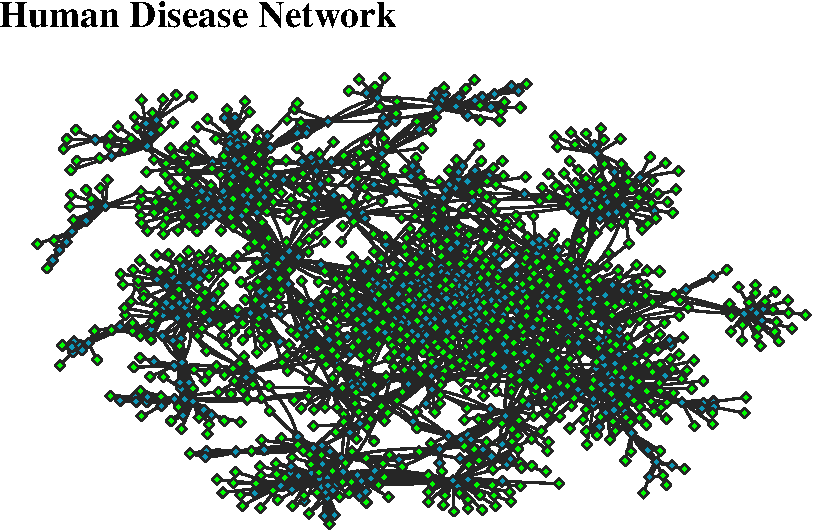
\includegraphics{HumanDiseaseNetwork_files/figure-latex/graph-1.pdf}

In this graph, genes are highlighted in Green, while diseases are highlited in Blue. It's possible to see that the network is quite wide, consisting of more than 3000 nodes and more than 1000 vertices.
the gene class is also more represented than the disease one, presenting two times the number of gene. It's also important to note that we are working with a directed graph.

\begin{verbatim}
## [1] "Vertices Number: 1419"
\end{verbatim}

\begin{verbatim}
## [1] "Genes Number: 903"
\end{verbatim}

\begin{verbatim}
## [1] "Diseases Number: 516"
\end{verbatim}

\begin{verbatim}
## [1] "Edges Number: 3926"
\end{verbatim}

\hypertarget{centrality-analisys}{%
\section{Centrality Analisys}\label{centrality-analisys}}

\hypertarget{degree-centrality}{%
\subsection{Degree Centrality}\label{degree-centrality}}

giving the fact that the graph is a directed graph, analisys over degree will take count of Outdegree and Indegree for a certain node, cause in the case of a directed graph both are present. Nodes with high degree will be considered as Hubs for the network, and the idea is that they will be central in clusters. values for degree centrality are normalized.

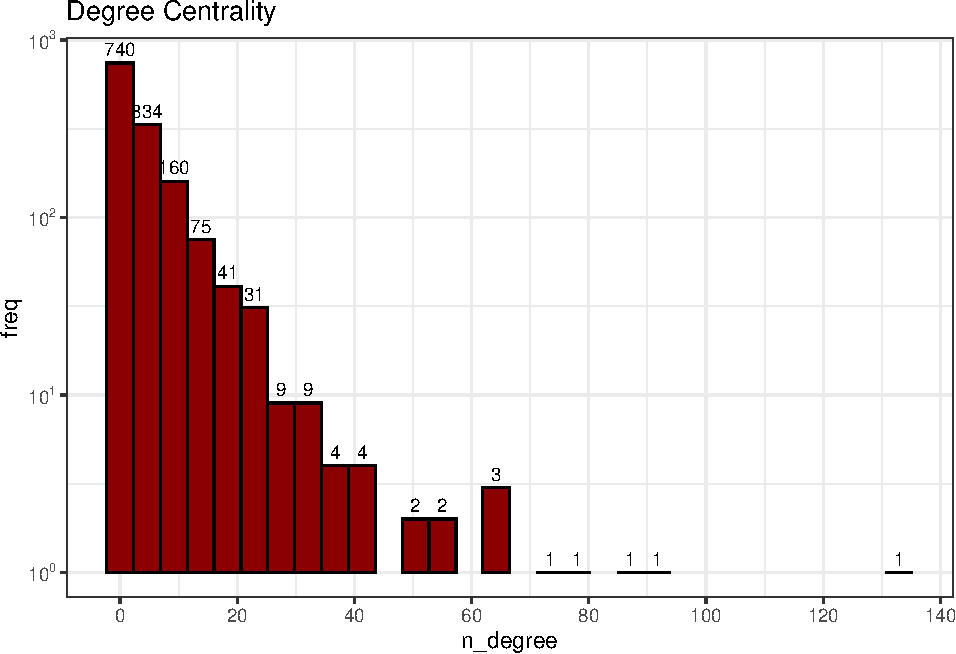
\includegraphics{HumanDiseaseNetwork_files/figure-latex/unnamed-chunk-4-1.pdf}

analyzing the results, it's clear that a lot of nodes have a centrality value close to 1, and, given the number, it's fair to say that genes are the main cause of this behaviour cause the majority of them have 1 as degree.

\begin{verbatim}
## `stat_bin()` using `bins = 30`. Pick better value with `binwidth`.
## `stat_bin()` using `bins = 30`. Pick better value with `binwidth`.
\end{verbatim}

\begin{verbatim}
## Warning: Transformation introduced infinite values in continuous y-axis

## Warning: Transformation introduced infinite values in continuous y-axis
\end{verbatim}

\begin{verbatim}
## Warning: Removed 10 rows containing missing values (geom_bar).
\end{verbatim}

\begin{verbatim}
## Warning: Removed 10 rows containing missing values (geom_text).
\end{verbatim}

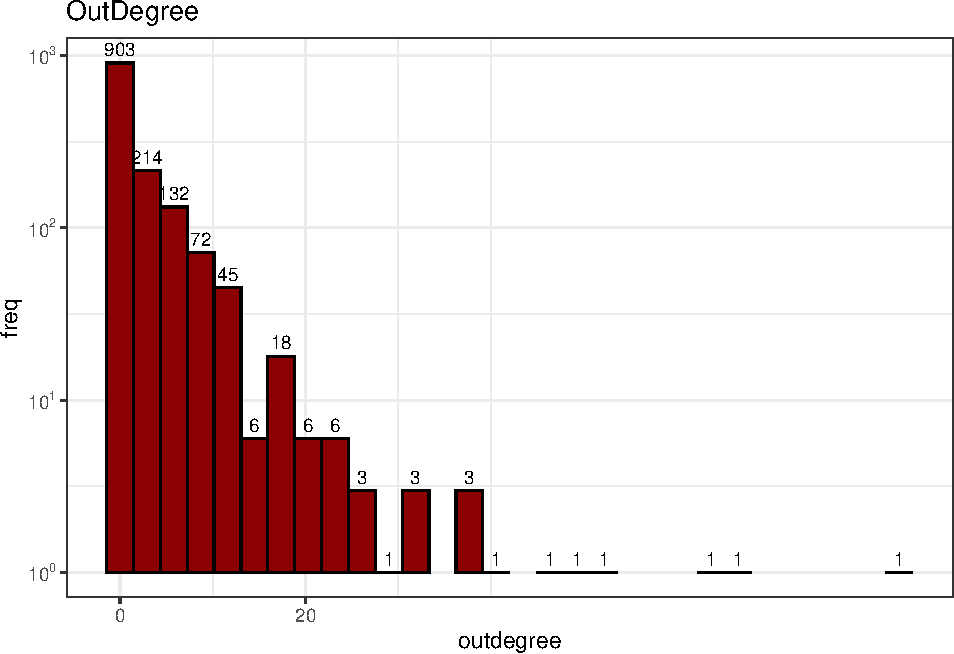
\includegraphics{HumanDiseaseNetwork_files/figure-latex/unnamed-chunk-5-1.pdf}

\begin{verbatim}
## `stat_bin()` using `bins = 30`. Pick better value with `binwidth`.
## `stat_bin()` using `bins = 30`. Pick better value with `binwidth`.
\end{verbatim}

\begin{verbatim}
## Warning: Transformation introduced infinite values in continuous y-axis
\end{verbatim}

\begin{verbatim}
## Warning: Transformation introduced infinite values in continuous y-axis
\end{verbatim}

\begin{verbatim}
## Warning: Removed 15 rows containing missing values (geom_bar).
\end{verbatim}

\begin{verbatim}
## Warning: Removed 15 rows containing missing values (geom_text).
\end{verbatim}

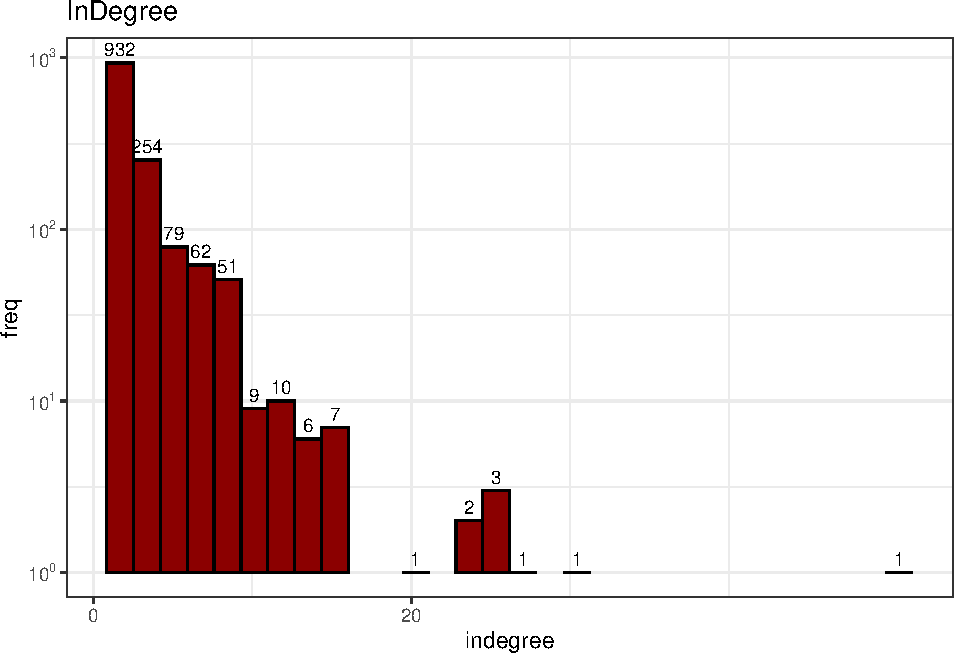
\includegraphics{HumanDiseaseNetwork_files/figure-latex/unnamed-chunk-5-2.pdf}

looking specifically at indegree numbers and outdegree numbers, it's possible to see that no one of the genes present an outgoing edge, and they just have one entering edge. it's now presented a rank of the top and bottom 10 nodes for degree.

\begin{verbatim}
## [1] "TOP 10 NODES FOR DEGREE"
\end{verbatim}

\begin{verbatim}
##  [1] "Colon cancer"         "Deafness"             "Leukemia"            
##  [4] "Breast cancer"        "Diabetes mellitus"    "Gastric cancer"      
##  [7] "Thyroid carcinoma"    "Retinitis pigmentosa" "Cardiomyopathy"      
## [10] "Pancreatic cancer"
\end{verbatim}

\begin{verbatim}
## [1] "BOTTOM 10 NODES FOR DEGREE"
\end{verbatim}

\begin{verbatim}
##  [1] "MTP"   "CNGA3" "GNAT2" "SSTR5" "PLAG1" "OCA2"  "TYRP1" "GFAP"  "A2M"  
## [10] "APBB2"
\end{verbatim}

as expected from the histograms, all the top 10 nodes are diseases, while all the bottom 10 are genes.

\hypertarget{betweenness}{%
\subsection{Betweenness}\label{betweenness}}

Betweenness is a measure that represents how central is a node based on how many shortest paths on the totality of them present the selected node. this is a more robust metric to evaluate centrality of a node because is not only based on the node itsefl. The measure is calculated in his normalized variant.

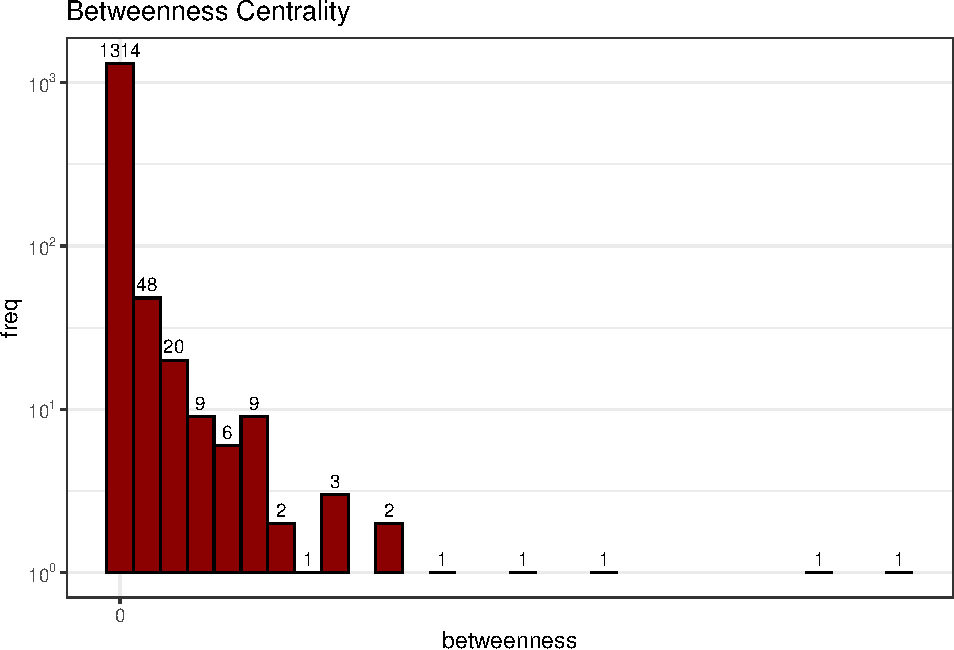
\includegraphics{HumanDiseaseNetwork_files/figure-latex/unnamed-chunk-7-1.pdf}

as for the degree measure, a lot of nodes sits on a low value of betweenness. just 5 of the nodes have a quite higher value of Betweenness, and it's expected that they will be hubs.
Those are the top nodes for Betweenness:

\begin{verbatim}
##  [1] "Cardiomyopathy"    "Lipodystrophy"     "Diabetes mellitus"
##  [4] "Glioblastoma"      "Deafness"          "Myopathy"         
##  [7] "Cataract"          "Leukemia"          "Colon cancer"     
## [10] "Alzheimer disease"
\end{verbatim}

\hypertarget{closeness}{%
\subsection{Closeness}\label{closeness}}

\end{document}
